\documentclass{article}
\usepackage{graphicx}
\usepackage{hyperref}
\usepackage{listings}
\usepackage{xcolor}
\usepackage{amsmath}

% Define code styling
\lstdefinestyle{pythonstyle}{
    language=Python,
    basicstyle=\ttfamily\small,
    keywordstyle=\color{blue},
    commentstyle=\color{gray},
    stringstyle=\color{red},
    breaklines=true,
    frame=single
}

\title{HxF User Manual: A Pebble Bed Reactor Simulation Tool}
\author{Ludovic Jantzen}
\date{\today}

\begin{document}

\maketitle
\tableofcontents
\newpage
\section{Introduction}
This document serves as a user manual for the Pebble Bed Reactor (PBR) simulation tool, HxF. The primary purpose of this tool is to perform high-fidelity simulations of PBRs, providing pebble-wise results. Unlike traditional zone-averaged approaches, HxF computes the neutron flux, power, and isotopic concentrations for each individual pebble within the reactor. Additionally, it depletes each pebble separately and manages pebble circulation.

The tool incorporates two motion models:
\begin{itemize}
\item Discrete Motion (DM): Simulates pebble movement by swapping compositions on a static lattice structure. This approach is particularly suited for simple geometries, such as the gFHR.
\item Discrete Element Method (DEM): Incorporates continuum mechanics equations to compute the forces acting on each pebble, accounting for small deformations. This method is not included within HxF itself; instead, externally generated pebble positions must be provided as input.
\end{itemize}

HxF offers additional features, such as the ability to account for different pebble types and implement various discard criteria based on either the number of passes or the accumulated burnup.

This tool is particularly useful for determining the equilibrium state of a reactor while obtaining detailed pebble-wise lifecycle data.

The tool relies mainly on the MC code Serpent 2 \cite{Serpent} and especially a modifed version to handle pebble geometry contruction and specific domain decomposition for PBR. Moreover, the dynamic interaction with Serpent is fostered thanks to the Cerberus/Kraken Python framewrok. See more here: \url{https://serpent.vtt.fi/kraken/index.php?title=Main_Page}. These tools help to dynamically interact with Serpent and handle Serpent input variables as Python variables.
\newpage
\section{Installation and Dependencies}
To use this tool, ensure you have the following dependencies installed:
\begin{itemize}
    \item Python 
    \item Required Python libraries:
    \begin{itemize}
        \item pandas
        \item numpy
        \item matplotlib
        \item cerberus
    \end{itemize}
\end{itemize}

The Cerberus library can be found on the the cluster storage under the path: 
\begin{verbatim}
/global/home/groups/co_nuclear/HxF_tools/Cerberus_HxF
\end{verbatim}

The first step will be to clone the given github repository.
Clone the repository:
\begin{lstlisting}[style=pythonstyle]
git clone https://github.com/ludojantzen/HxF.git
\end{lstlisting}

It's recomanded to clone it in a location where the simualtion will have enough memory to store results (such as \texttt{scratch} space for example)

\newpage
\section{Repository Structure}

This section describes the organization of the repository, outlining the key directories and files that compose the simulation framework for the Pebble Bed Nuclear Reactor. The repository is structured to facilitate ease of use, modification, and extension of the simulation capabilities.

The HxF repository is organized as follows:

\begin{verbatim}
HxF/
├── Input_scripts/
├── Models/
├── Source/
├── Tools/
├── Utils/
├── HxF.py
├── README.md
├── config/
└── launch_HxF

\end{verbatim}

\begin{itemize}
    \item \texttt{Input\_scripts/}: Contains input scripts for simulations. It takes the form a python script providing the main simulation parameters such as the motion mode, the pebble types and the discardiung threshold. This will be decsribe in the section 
    \item \texttt{Models/}: Stores various reactor models used in simulations, gFHR, HTR-10, small PBR.
    \item \texttt{Source/}: Includes the source code of the HxF tool. These files should be left as they are because they have been built to simulate and plot general PBR related stuffs. 
    \item \texttt{Tools/}: Provides auxiliary tools and utilities. Useless for basic applications. Contains some tools for detection and ML purposes.
    \item \texttt{Utils/}: Contains utility scripts and functions. Really helpfull for permanent environment setup and LSURM environment creation and variable exportation (Serpent envirionment, module loading). Please check the section \ref{sec:set_up_env}.
    \item \texttt{HxF.py}: The main Python script to run the HxF tool. Please check section \ref{sec:HxF}
    \item \texttt{README.md}: Documentation and overview of the HxF project.
    \item \texttt{config}: configuration file. It helps to configure the SLURM job (ressource, computational time, partition... see section \ref{sec:config}
    \item \texttt{launch\_HxF}: Script to launch HxF simulations. Submit the job for you with all the needed info: Input scripts, environment... see section \ref{sec:launch}
\end{itemize}

Additionally, HxF while running will create a directory \textbf{Cases/} and a directory \textbf{Logs/}. This two directories will contain the outputs and the log files from Serpent and the cluster, 
\newpage

\section{Code Structure and Simulation Loop}

The HxF tool operates in a sequential loop to simulate the evolution of a Pebble Bed Reactor (PBR). Usually, the user will set a total number of iterations. In addition, the iteration corresponds to an actual time-step  Each iteration consists of the following steps:

\begin{enumerate}
    \item \textbf{Neutron Transport:} Compute the flux and power distribution for each pebble in a static bed.
    \item \textbf{Burnup Calculation:} Deplete each pebble individually based on the previously computed neutron flux. The burnup step duration matches the motion step duration.
    \item \textbf{Pebble Motion:} Move the pebbles according to the selected motion model (Discrete Motion or Discrete Element Method).
    \item \textbf{Pebble Handling:} After motion, the tool manages the discard, discharge, and reinsertion of pebbles. New pebbles are reinserted with random radial positions. You can also apply a artificial decay time corresponding to a potential 
\end{enumerate}

For instance, let say that your time step is 3 days between two iterations. It means that your burnup step will be 3 days and that your sequential motion step will correspond to three days of continuous motion.

This iterative process continues until you reach the predefined number of simulated step. Some features propose to stop the simulater based on certain criteria such as the variation in the multiplication factor. The overall flexibility of the Python tool allows for you to define your own convergence criteria as long as it's related to a Serpent output value.

Generally, in figure \ref{fig:HxF}, you can find the overall workflow for HxF. A thermal coupling block is interacting with the transport calculation is pointted out and discussed in the Appendix \ref{sec:TH}. 

\begin{figure}[] 
    \centering
    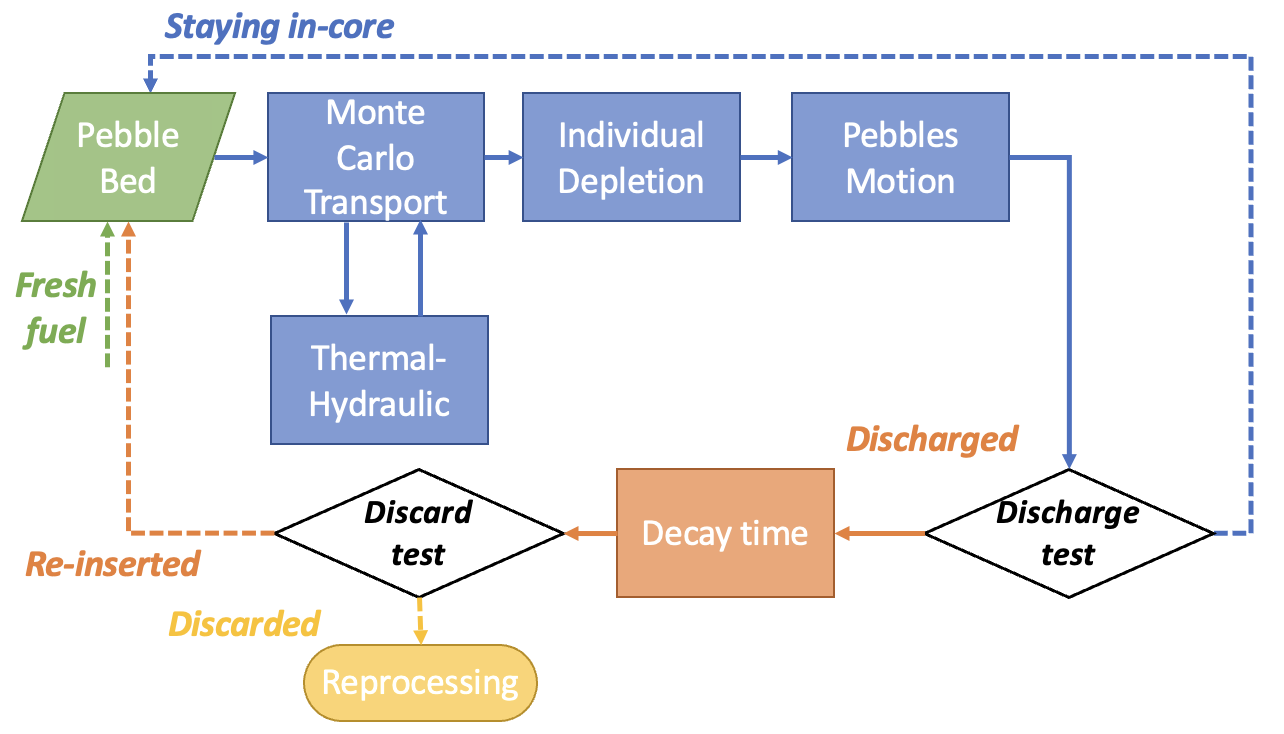
\includegraphics[width=1\textwidth]{Figures/HxF.png}
    \caption{HxF workflow \cite{Yves_HxF}.}
    \label{fig:HxF}
\end{figure}

\clearpage
\section{Setup and Environment Configuration}\label{sec:set_up_env}
\subsection{Setting Up Cerberus: The \texttt{setup\_Cerberus} Script}
The \texttt{setup\_Cerberus} script is a crucial component for configuring the environment required to run the simulation tool. It ensures that all necessary dependencies are installed and properly configured before executing any simulations. This script should be executed once before using the tool for the first time.

\subsubsection{Purpose and Impact}
The script automates the setup of the computing environment, handling:
\begin{itemize}
    \item Unloading conflicting software modules and loading required ones.
    \item Installing and configuring Miniconda if it is not already present.
    \item Creating a dedicated Conda environment for running the simulation.
    \item Installing necessary Python packages and dependencies.
    \item Ensuring compatibility with Cerberus and KrakenTools frameworks.
\end{itemize}

\subsubsection{Step-by-Step Breakdown}
The script follows these main steps:

\paragraph{1. Module Management}  
To prevent software conflicts, the script first unloads any existing Python, GCC, CMake, and Nano modules before loading the correct versions required for the simulation.

\paragraph{2. Miniconda Installation}  
If Miniconda is not found in the user's home directory, the script downloads and installs it. This ensures a controlled Python environment without affecting system-wide installations.

\paragraph{3. Creating a Custom Conda Environment}  
The script configures a Conda environment named \texttt{kraken}, placing it in the scratch directory to optimize storage usage. It also configures Conda to store package installations in a designated location.

\paragraph{4. Installing Dependencies}  
Within the new Conda environment, the script installs essential Python libraries such as:
\begin{itemize}
    \item \texttt{serpentTools} for processing Serpent Monte Carlo outputs.
    \item \texttt{numpy, scipy, pandas} for numerical and data manipulation.
    \item \texttt{matplotlib, seaborn} for visualization.
    \item \texttt{mpi4py} for parallel computing.
\end{itemize}

\paragraph{5. Linking Cerberus and KrakenTools}  
To ensure proper integration with the simulation framework, the script links the Cerberus and KrakenTools directories to the Conda environment.

\paragraph{6. Verification}  
Finally, the script deactivates and reactivates the environment to confirm that Cerberus is correctly installed by running a simple import test.

\subsubsection{Execution}
To set up the environment, run:
\begin{lstlisting}
bash ./Utils/setup_Cerberus
\end{lstlisting}
This should only be run once before using the simulation tool. If any updates are made to the environment, re-executing the script ensures a clean and correct setup.


\subsection{Activating Kraken: The \texttt{sss\_environment} Script}
The \texttt{sss\_environment} helps you to load the correct simulaiton for your coming simulation, export the good serpent path and activate kraken, the environment used to run the searc\_equilibrium tool.


\subsection{Testing the environment and kraken activation}\label{sec:Cerberus}

After sourcing the \texttt{sss\_environment} script, you should be able to do a few checks. The first one will be to see what is the current path related to the accessible python module: 
\begin{verbatim}
[ludovicjantzen@ln002 search_equilibrium]$ which python
/global/scratch/users/ludovicjantzen/conda/kraken/bin/python
\end{verbatim}

Then by running accessing the python throught the kraken environment: 

\begin{verbatim}
    

[ludovicjantzen@ln002 search_equilibrium]$ python
Python 3.11.11 | packaged by conda-forge |
(main, Mar  3 2025, 20:43:55) [GCC 13.3.0] on linux
Type "help", "copyright", "credits" or "license" for more information.
>>> import cerberus
>>> cerberus
<module 'cerberus' from '/global/home/groups/co_nuclear/
HxF_tools/Cerberus_HxF/cerberus/__init__.py'>
>>> 
\end{verbatim}
You should be able to import cerberus and access its location without error. This means that your kraken environment has been set up correctly.
\newpage
\section{Input Scripts}\label{sec:input_script}
This scetion explains the role of the input scripts. They take the form of a Python script where a few dozens of variables are defined. You can find a template under \texttt{HxF/Source
/Default\_Input.py}. It's also really valuable to spend time understanding the available example of input scripts available under \texttt{Input\_scripts}. Here you can find a quick explanation of all the options: 


\subsection{Calculation Options}
\begin{itemize}
    \item \textbf{transport}: Enables neutron transport calculations.
    \item \textbf{resolve\_first}: If true, performs an initial resolution step.
    \item \textbf{correct}: Applies correction methods if enabled. Basically turn on the absic linear pcc in Serpent. The use ot this method is still highly debated in PBR simulation since we overlap this metod with a motion scheme.
    \item \textbf{domain\_decomposition}: Activates domain decomposition for parallel execution. Decompose based on the number of requested nodes.
\end{itemize}

\subsection{Motion Settings}
\begin{itemize}
    \item \textbf{discrete\_motion}: Enables discrete motion model (DM). If set to False, the DEM positions should be provided.
    \item \textbf{looping}: If true, enables looping motion mode. This technic is compatible with DEM calculation where HxF will match the pebble positions between the first and the last position data set. It helps to simulate long circulation sequences while simulating a handful series of positions 
\end{itemize}

\subsection{Restart Settings}
\begin{itemize}
    \item \textbf{restart\_calculation}: If true, starts from a previously saved state. To restart the calculaiton, you'll need two type of files. The dataFrame containing the pebble positions named \texttt{core\_step.csv} and the Serpent restart file containing the pebble composition. Usually, you restart a HxF calculation with previous HxF results.
    \item \textbf{read\_first\_compositions}: Reads initial compositions from predefined files for each pebble.
\end{itemize}

\subsection{Output Settings}
\begin{itemize}
    \item \textbf{plotting}: Enables visual output of results. These plot are stored in the folder \textbf{Cases/your\_case/} and are generated at each calculation step. See more in section \ref{sec:cases}.
    \item \textbf{saving}: Saves results to disk.
    \item \textbf{write\_restart}: Enables writing restart files.
\end{itemize}

\subsection{Case Information}
\begin{itemize}
    \item \textbf{path\_to\_case}: Directory where the Serpent input files are stored. Usually, it's stored under \textbf{Models/}.
    \item \textbf{case\_name}: Name of the case. This name is informative and will be used to name the log file. 
    \item \textbf{main\_input\_file}: Name of the main Serpent input file.
\end{itemize}

\subsection{Serpent Input Data}
\begin{itemize}
    \item \textbf{pbed\_file}: Pebble position file. This is particularly important when using the Discrete Motion (DM) model, where pebbles follow a structured lattice. In this case, the position file serves as a reference for the simulation, and the DM tool updates pebble compositions accordingly without altering their spatial arrangement.
    \item \textbf{r\_pebbles}: Pebble radius (cm).
\end{itemize}

A crucial part of the input configuration is the \texttt{pebbles\_dict}, which defines the properties of different pebble types. For example, the following dictionary describes the HTR-10 configuration:

\begin{verbatim}
    pebbles_dict = {'u_fuel_pebble':{'mat_name':'fuel', 'pebbles_frac':0.57,
    'r_fuel_kernel':0.025, 'Ntrisos':8335, 'threshold_type':'burnup',
    'threshold_dir':+1, 'threshold':72},
                'u_graph_pebble':{'pebbles_frac':0.43}}
\end{verbatim}

Each entry in this dictionary corresponds to a specific universe defined in the Serpent input (\texttt{u\_fuel\_pebble} and \texttt{u\_graph\_pebble}). The parameters for each universe are as follows:

\begin{itemize}
    \item \textbf{mat\_name}: Material name (only required for burnable pebbles).
    \item \textbf{pebbles\_frac}: Fraction of this type of pebble in the core (e.g., in the HTR-10, 57\% of the pebbles are fuel pebbles).
    \item \textbf{r\_fuel\_kernel}: Fuel kernel radius (cm).
    \item \textbf{Ntrisos}: Number of TRISO particles per fuel pebble (used to compute the fuel volume).
    \item \textbf{threshold\_type}: Criterion for discarding pebbles (e.g., \texttt{burnup}, \texttt{passes}, or isotope concentration).
    \item \textbf{threshold\_dir}: Direction of the threshold check (\texttt{+1} for exceeding the threshold, \texttt{-1} for falling below it).
    \item \textbf{threshold}: Numeric value defining the discard limit (e.g., fuel pebbles in the HTR-10 are discarded when their burnup exceeds 72 MWd/kgHM).
\end{itemize}

You can also add pebble-wise detectors with this format: 
\begin{verbatim}
    detectors = {'flux_pebbles_thermal':{'E':[1e-11, 1.86e-6],
    'normalized':True},
             'flux_pebbles_fast':{'E':[0.18, 20], 'normalized':True},
             'power_pebbles':{'extra_cards':['dr', -8, 'void']}}
\end{verbatim}

Moreover, HxF integrates an integration process deriving fluence from flux and energy from power (time integration over the entire pebble life-cycle).

Different threshold criteria can be used for pebble discard decisions, such as the number of passes through the core, accumulated burnup, or the mass fraction of specific isotopes (Cs-137). For a more comprehensive discussion of available discard criteria, refer to Section~\ref{sec:cases}.


\subsection{Transport Calc Settings}
\begin{itemize}
    \item \textbf{power\_normalization\_field}: Field used for power normalization.
    \item \textbf{power\_normalization\_value}: Total reactor power (W).
    \item \textbf{Nsteps}: Number of calulation steps. Usually, we use a high number of steps ($\sim$ 1000). The cluster time-limit of 3 days will cut-off this high number of stesp but at least you're sure your simulation as far as possible.
    \item \textbf{neutrons\_per\_cycle}: For each single simulation step, you can define the number of simulated neutrons. this number will be the same assigned to active and inactive cycle of a given HxF calculation step. Regarding the number of active and nactive cycle, these parameters are defined in the Serpent input in \textbf{Models/} with the classic card \texttt{set pop}. 
    
    Since you define the number of neutrons for each computation step, \texttt{neutrons\_per\_cycle} should be a list with a lentgh of \texttt{N\_steps}. The common practice is to use a low number of neutrons to approach equilibrium and then refine when the equilibrium is reached. Example:
    \begin{verbatim}
         neutrons_per_cycle=[20000]*68*2+[500000]*(Nsteps-68*2)
    \end{verbatim}
    \item \textbf{decay\_step}: Decay step applied to every discharged pebble to simulate the off-core time. Most of the time set to 0 because the recirculation time ends up being really short ($\sim$ 5 minutes). 
\end{itemize}

\subsection{Motion Parameters for DM}
Discrete Motion (DM) follows predefined movement rules per step, controlling the pebble flow in the reactor. The key parameters for DM are:

\begin{itemize}
    \item \textbf{motion\_direction}: Defines the movement direction (+1 or -1).
    \item \textbf{Nrows\_to\_move}: Number of pebble rows moved per step.
    \item \textbf{time\_per\_pass}: Time per pass (days) in discrete motion mode. Similar to \texttt{neutrons\_per\_cycle}, this parameter is a list with a length equal to \texttt{N\_steps}. It influences both the motion increment and the burnup step size. The time step is refined once equilibrium is reached to improve accuracy.

\begin{verbatim}
    Nrows_to_move = [6]*68*2 + [3]*(Nsteps-68*2)
\end{verbatim}

\end{itemize}

\subsection{Motion Parameters for DEM}
The Discrete Element Method (DEM) relies on externally generated position files, typically named \texttt{position\_step.csv}, which must be accessible when launching HxF. The parameters controlling DEM-based motion include:

\begin{itemize}
    \item \textbf{recirc\_threshold}: Threshold for recirculation (cm). HxF detects pebble recirculation by comparing axial positions between consecutive DEM steps. If the absolute displacement exceeds this threshold, the pebble is considered to have recirculated.
    \item \textbf{positions\_folder}: Directory containing DEM-generated position files.
    \item \textbf{DEM\_step\_increment}: Defines the step increment when reading position files. A value of 1 means all files are used, while 2 means every other file is used.
    \item \textbf{circulation\_rate}: Pebble circulation rate (pebbles per day).
    \item \textbf{DEM\_circulation\_step}: Number of pebbles per DEM circulation step.
    \item \textbf{positions\_scale}: Scaling factor for DEM positions.
    \item \textbf{positions\_translation}: Translation vector for DEM positions. Since Serpent's reactor geometry must align with the DEM-generated positions, this translation ensures consistency.
    \item \textbf{looper\_Nr, looper\_Nz, looper\_method}: Parameters for the looping method. Details on available looping methods can be found in \texttt{./Source/Looping.py}.
\end{itemize}

\subsubsection{Example: HTR-10 Configuration}
In this example, the DEM-generated positions cover 90 steps, with each step corresponding to a time increment of 12.5 days. The following input parameters apply:

\begin{verbatim}
    recirc_threshold = 200 # cm
    positions_folder = '/global/scratch/users/co_nuclear/pebble_positions_larger/'
    DEM_step_increment = 1
    circulation_rate = 125 # pebbles/day
    DEM_circulation_step = 1564 # pebbles
    positions_scale = 100
    positions_translation = [0, 0, -610]
    
    if looping:
        DEM_start = 40
        DEM_end = 129
        looper_Nr = 5
        looper_Nz = 10
        looper_method = 'rz'
\end{verbatim}

\textbf{Explanations:}  
A large recirculation threshold is set to detect full pebble recirculations. In the HTR-10, recirculated pebbles move from $z=-610$ cm to $z=0$ cm. The \texttt{circulation\_rate} and \texttt{DEM\_circulation\_step} indicate that the DEM time step is around 12.5 days. Since the DEM outputs positions in meters while Serpent expects centimeters, the \texttt{positions\_scale} corrects for unit differences. Additionally, the DEM simulation spans $z=0$ m to $z=6.10$ m, whereas the Serpent geometry spans $z=-610$ cm to $z=0$ cm, justifying the need for \texttt{positions\_translation}.
When looping is enabled, HxF applies a repeating pattern to DEM positions. The looping parameters are:
\begin{itemize}
    \item \textbf{looper\_Nr}: Number of radial divisions.
    \item \textbf{looper\_Nz}: Number of axial divisions.
Indeed, the looper assigned the positions per block that are built from the subdivision defined with \textbf{looper\_Nz} and \textbf{looper\_Nr}. More detail about the looping tool and the induced error is discussed in \cite{Yves_M&C}.
    \item \textbf{looper\_method}: Defines how looping is applied. Available methods include:
    \begin{itemize}
        \item \textbf{'rz'}: Minimize r and z distance between the old and new position.
        \item \textbf{'xyz'}: Minimize the distance between the old and the new position.
    \end{itemize}
\end{itemize}

\subsection{Output and Data Storage}
\begin{itemize}
    \item \textbf{output\_folder\_name}: Directory where output files are stored in the directory \textbf{Cases/}. It's really important to set this name correctly and rememebr to cahnge to not overwrite the previous results.
    \item \textbf{verbosity\_mode}: Level of verbosity for logging.
    \item \textbf{inventory\_names}: List of isotopes tracked in inventory calculations. These isotopes will end up being stored at the pebble wise level for each step in the \texttt{core\_{step}.csv} file. For instance, this isotope inventory can be used as a discard threshold.
\end{itemize}

\subsection{Domain Decomposition}
\begin{itemize}
    \item \textbf{allowed\_decomposition\_types}: Types of domain decomposition allowed.
    \item \textbf{max\_domains}: Maximum number of subdomains.
\end{itemize}

More details are given in the section \ref{sec:dd}

\subsection{Restart Writing}
\begin{itemize}
    \item \textbf{restart\_write\_every}: Frequency (in steps) for writing core composition restart files.
    \item \textbf{restart\_discarded\_write\_every}: Frequency (in steps) for writing discarded composition restart files.
    \item \textbf{restart\_discharged\_write\_every}: Frequency (in steps) for writing discharged composition restart files.
\end{itemize}

\subsection{Restart Reading}
\begin{itemize}
    \item \textbf{restart\_step}: Step number from which to restart.
    \item \textbf{restart\_data}: Path to restart data file. It corresponds to the file {core\_{step}.csv}.
    \item \textbf{restart\_binary}: Path to restart binary file. It corresponds to the Serpent restart binary file.
\end{itemize}

\subsection{Saving Options}
\begin{itemize}
    \item \textbf{write\_global}: Saves global reactor data.
    \item \textbf{write\_incore}: Saves data of pebbles inside the core.
    \item \textbf{write\_reinserted}: Saves data of reinserted pebbles.
    \item \textbf{write\_discarded}: Saves data of discarded pebbles.
    \item \textbf{write\_discharged}: Saves data of discharged pebbles.
\end{itemize}

This detailed parameter list provides an overview of the key input settings in HxF. These options allow users to customize the simulation workflow, neutron transport, depletion, motion, and output settings.

\subsection{Final note}

We saw the main general options available. Obviously, if your options are not well spelled or does not exist, the script will return you an error. There is a section in the appendix that explains how to test your code before submintting your job. In addition, if ou want to double check the role of a specific parameter or its availability, the best is to look directly at the script \texttt{HxF.py}. 

\newpage
\section{Models}\label{sec:models}
This section describe the \textbf{Models} folder. It contains the Serpent input. Usually, it required the definition of the reactor geometry, the reactor materials. Then, regarding the simulation parameters such as power normalization, neutron pouplation, burnup step..., all these parameters will be write down by the tool directly, or set as dynamic variables thanks to Cerberus. The process that HxF is doinf is to first delete all the redoundant information in the Serpent input, collect the necessary information such as reactor geometry, reference pebble positions for the DM tool, material composition... and then add the needed simulation parameters derived from the Python input scripts. 

The repository contain a few reactor models:
\begin{itemize}
\item the gFHR and some more complex models derived from the base model that is referenced here \cite{gFHR}. It's a simplified generic benchmark recator for neutronic calculation featuring a purely cylindrical shape. The base model involves a DM tool with a FCC structure as a posiotion refrences. gFHR core has been simulated also involving DEM position determination. Also, a model with a more complex geometry featuring conical regions and fueling/defueling chute under the directory \textbf{Models/gFHR\_cone/}, also simulated with DEM tool.

\item the HTR-10 which is a benchmark recator built in China in 2000 to demonstrate the feasability of helium-cooled PBR. The main reactor parameters can be found in \cite{INL_report_HTR-10}. This reactor features a complex geometry that requires to use the DEM tool. Some variations of this model can be found such as a longer core to fit more pebbles. Usually, we only use the main model under \textbf{Models/HTR-10/}. This model still includes some specificities such as two types of pebbles, fule and graphite pebble. The fraction of each of these pebbles usually allows to reach criticallity at equilibrium. 

\item the small PBR is a smaller version of the gFHR, scalled down for test purposes. It produces 5 MWth. 


\end{itemize}
\newpage
\section{The script \texttt{HxF.py}}\label{sec:HxF}
The script \texttt{HxF.py} is the main script executing your Python input script. The code can be seperated in a few sections:
\begin{itemize}
    \item First section is about importing modules, especially the Cerberus module. 
    \item Then the code modifies the provided Serpent input and add the required parameters derived from the Python input.
    \item The code initialize the simulation environment by creating dynamic variables thanks to the Cerberus/Kraken.
    \item The loop aver the total number of calculation strps that operates transport, brunp and pebble motion.
\end{itemize}

\newpage
\section{The script \texttt{config}}\label{sec:config}

\subsection{HxF Execution Script}
The following Bash script automates the execution of HxF on a computing cluster, ensuring the correct setup of Python and Serpent environments while handling cluster-specific configurations.

\subsubsection{Script Breakdown}
This script defines and manages the execution of an HxF simulation with the following key components:

\begin{itemize}
    \item \textbf{Python Scripts:}  
    The script specifies the input Python file (\texttt{HTR10\_coupled.py}) and the main HxF execution script (\texttt{HxF.py}), which should not be modified.

    \item \textbf{Conda Environment:}  
    The script activates the Conda environment \texttt{kraken}, which was set up using \texttt{setup\_Cerberus}. Additionally, the script sources \texttt{sss\_environment}, ensuring all necessary environment variables are loaded.

    \item \textbf{Cluster Configuration:}  
    The script is designed to run on a high-performance computing (HPC) cluster, defining:
    \begin{itemize}
        \item \texttt{GROUP\_ACCOUNT}: Account name (e.g., \texttt{fc\_neutronics} or \texttt{co\_nuclear}).
        \item \texttt{PARTITION}: HPC partition (e.g., \texttt{savio3}).
        \item \texttt{NNODES}: Number of nodes allocated for the job.
        \item \texttt{QOS}: Quality of Service setting for resource allocation.
        \item \texttt{NHOURS}: Maximum runtime in hours.
        \item \texttt{SUFFIX\_JOB}: Optional suffix for job naming.
    \end{itemize}

    \item \textbf{Serpent Configuration:}  
    The script specifies paths and libraries needed to run Serpent:
    \begin{itemize}
        \item \texttt{SERPENT\_EXE}: Path to the Serpent executable.
        \item \texttt{SERPENT\_DATA}: Directory containing nuclear data files.
        \item \texttt{SERPENT\_ACELIB}, \texttt{SERPENT\_DECLIB}, \texttt{SERPENT\_NFYLIB}: Paths to cross-section, decay, and fission yield libraries.
    \end{itemize}

    \item \textbf{OpenFOAM Configuration:}  
    The script sets \texttt{OF\_BASHRC}, which loads the OpenFOAM environment for coupled simulations. This is only needed if you run a coupled simulation. In the Appendix \ref{sec:TH}, there is a quick discussion about the TH coupling, its feasibility and its interest.
\end{itemize}

This script ensures that all dependencies are correctly set before executing HxF, facilitating seamless integration of Python, Serpent, and OpenFOAM simulations on an HPC cluster.

Note: Any cluster realted issues such as bad combinations of cluster paramters may be solved refering to the Savio user manual. Moreover, the Serpent and XS libraries are usually updated continuously and these modification should be reflected in your \texttt{config} file.

\newpage
\section{The script \texttt{launch HxF}}\label{sec:launch}

\subsection{HxF Job Submission Script}
This script is responsible for configuring and submitting HxF simulations on an HPC cluster using SLURM. It ensures that all necessary environment variables are set up correctly before launching the job.

\subsubsection{Script Breakdown}
This script automates job submission for HxF simulations and ensures the correct SLURM configuration.

\begin{itemize}
    \item \textbf{Configuration Loading:}  
    The script requires a configuration file as an argument and sources it, ensuring all environment variables are set.

    \item \textbf{Environment Variables Export:}  
    Essential environment variables such as Python script names, SLURM job details, and Serpent configurations are exported for use in the job execution.

    \item \textbf{SLURM Parameters:}  
    \begin{itemize}
        \item \texttt{PARTITION\_CPUS\_PER\_NODE}: Dynamically fetches the maximum number of CPUs per node for the selected partition.
        \item \texttt{SUFFIX\_JOB}: Appends a suffix to the job name if specified.
        \item \texttt{JOB\_NAME}: Generates a job name based on the input script filename.
        \item \texttt{OUTPUT\_FILE}, \texttt{ERROR\_FILE}: Log files are created under \texttt{./Logs/}.
        \item \texttt{TIMELIMIT}: Converts the requested job time (\texttt{NHOURS}) into HH:MM:SS format.
    \end{itemize}

    \item \textbf{Data Cleanup:}  
    Ensures that unset Serpent variables are removed to prevent incorrect configurations.

    \item \textbf{Job Execution and Logging:}  
    The script prints all job-related parameters for verification before submitting the job using \texttt{sbatch}. The \texttt{Utils/exe.sub} script is executed, running the simulation in the allocated SLURM environment.
\end{itemize}

This script streamlines the execution of HxF on an HPC system by automating the job submission process and ensuring robust configuration management.

Now looking at the \texttt{exe.sub}, we can summarize the role of this file. The script launch the job with the cluster parameters defined in \texttt{config}. 

The few commands that the cluster has to execute are the follwoing:
\begin{lstlisting}[style=pythonstyle]
    #!/bin/bash

# Load the environment
source ${CONFIGURATION_FILE} ${CONDA_ENVIRONMENT}
if [ -n "$OF_BASHRC" ]; then
    source $OF_BASHRC
fi
# Run the Python script
mpirun -np 1 --report-bindings --bind-to none -oversubscribe 
python ${PYTHON_SCRIPT} ${INPUT_SCRIPT} ${PARTITION_CPUS_PER_NODE} ${NNODES}
\end{lstlisting}

This bash script load the environment (kraken) and export all the required variable for the cluster. Then it launches the python trhough a mpirun command. Basically, Cerberus will take as input the \textt{PARTITION\_CPUS\_PER\_NODE} and \textt{NNODES}, and spawn the MPI processes through the booked nodes. In this mode, it corresponds to the command:
\begin{verbatim}
    mpirun -np ${NNODES} Serpent.exe -omp ${PARTITION_CPUS_PER_NODE} 
    Serpent_input 
\end{verbatim}
So far, it has been the most memory efficient way to distribute the threads but can lead to some NUMA errors (ORTE DAEMON COMMUNICATION ERROR). 

\newpage
\section{The folder \textbf{Cases/}}\label{sec:cases}

The folder Cases will be created once you launch your first HxF simulation and store your updated Serpent input and your results under a specific directory that takes the name of the output folder name mentioned in the Python input scripts. Watch out: if you do not change the name of the output folder in the Python input script, you'll overwrite your previous results.

For each Case, you'll have a few types of results. You can first find the initial Serpent input that has been copied form the \textbf{Models} folder. It copies also your Python input to keep track of your simulation. Then you'll find three folders:
\begin{itemize}
    \item The folder \textbf{Data/} contains some pebble-wise data stored at each calculation step with the \texttt{.csv} format. There are a few types of file: \texttt{core\_{step}.csv}, \texttt{discharged\_{step}.csv},\texttt{discarded\_{step}.csv}, 
    \texttt{reinserted\_{step}.csv}, which respectively contain the pebble-wise information for the pebble in the core, discharged, discarded and reinsterted at step "\texttt{step}". The column of the files are the following ones in \texttt{core\_{step}.csv}: 
    \begin{verbatim}
Index(['Unnamed: 0', 'id', 'x', 'y', 'z', 'r', 'r_dist', 'row_id', 'uni',
       'mat_name', 'isactive', 'initial', 'insertion_step', 'avg_r_dist',
       'passes', 'recirculated', 'discarded', 'residence_time',
       'pebble_type_0', 'burnup', 'flux_pebbles_thermal',
       'flux_pebbles_thermal_rel_unc', 'integrated_flux_pebbles_thermal',
       'integrated_flux_pebbles_thermal_rel_unc',
       'integrated_flux_pebbles_thermal_unc', 'flux_pebbles_fast',
       'flux_pebbles_fast_rel_unc', 'integrated_flux_pebbles_fast',
       'integrated_flux_pebbles_fast_rel_unc',
       'integrated_flux_pebbles_fast_unc', 'power_pebbles',
       'power_pebbles_rel_unc', 'integrated_power_pebbles',
       'integrated_power_pebbles_rel_unc', 'integrated_power_pebbles_unc',
       'pass_residence_time', 'pass_agg_r_dist', 'pass_avg_r_dist',
       'pass_nsteps', 'pass_burnup', 'pass_integrated_flux_pebbles_thermal',
       'pass_integrated_flux_pebbles_thermal_unc',
       'pass_integrated_flux_pebbles_thermal_rel_unc',
       'pass_integrated_flux_pebbles_fast',
       'pass_integrated_flux_pebbles_fast_unc',
       'pass_integrated_flux_pebbles_fast_rel_unc',
       'pass_integrated_power_pebbles', 'pass_integrated_power_pebbles_unc',
       'pass_integrated_power_pebbles_rel_unc', 'domain_id'],
      dtype='object')
    \end{verbatim}
As you can see, pebble-wise information are really diverse. You can also see the pebble-wise results of the detectors and their corresponding time-integrated value (fluence for the flux). There are some details about pass-averaged value. 

Moreover, any \texttt{inventory\_names} defined in the Python input will be added as a pebble-wise atomic density value. You can also add some extra fields directly in your Python input setting up 
\texttt{extra\_fields=['fima', 'decayheat', 'activity', 'burnup']}.

Finally, in the \textbf{Data/} folder, you'll have a \texttt{cycle\_{step}.csv}. This file contains some general info about the simulation at each step. The file \texttt{cycle\_{step}.csv} includes all the concatenated info about each simgle step up to step \texttt{step}. The columns and available data are:
\begin{verbatim}
time,passes,recirculated,discarded,keff,keff_relative_uncertainty,
keff_absolute_uncertainty,neutrons_per_cycle,power_normalization_value,
DEM_step_increment,threshold_fuel,time_step
\end{verbatim}
\item The folder \textbf{Plots/} contains multiple plot for each calculation step such as \texttt{pass\_{step}.png}, \texttt{cumulative\_{step}.png}, \texttt{inventory\_{step}.png}, \texttt{keff\_{step}.png}. These file are generated only if the option top plot is selected in your Python input. 

\item The folder \textbf{wrk\_Serpent/} contains the updated Serpent input and all the usual Serpent input such as the \texttt{serpent\_res.m}, \texttt{serpent\_det\_{step}.m} and all the restart files for the core and potentially the discarded and discharged pebbles if the option has been selected to write all the restart files. 
\end{itemize}

Note: An additional folder \textbf{Logs/} is created and contains your logs. There are two logs outputed: 
\begin{itemize}
    \item \texttt{your\_job.o} is the HxF log containing the Serpent logs and the Cerberus log. In this log, you'll see where HxF script is failling and can return directly related Serpent error. 
    \item \texttt{your\_job.error} contains cluster error such as communication error, memory issues or environment problems. For cluster troubleshouting, please refer to the Savio user manual. 
\end{itemize}
\newpage
\section{Submiting your job}
The simple command to run will be:
\begin{verbatim}
    ./launch_HxF config
\end{verbatim}
In this case, \texttt{config} is the file used as an argument to launch the calculation. The reason why this file should be set up correctly before being launched. Please refered to the Savio user Manual to obtain the compatible partitions/accounts/QOS/time-limit/ressources. Since the HxF calculation can be restarted, reavhing the time limit is not a problem in itself. 


\newpage
\section{Parallel Computation}

\subsection{Overview}

HxF has been designed to model reactors ranging from small Pebble Bed Reactors (PBRs) with thermal power outputs of approximately 10 MWth to large-scale reactors containing over 100,000 pebbles. Simulating such large-scale systems requires both (1) a significant number of computational cores to accelerate the simulation process and (2) sufficient memory to handle burnup calculations. This is particularly relevant for HxF, which models the full reactor life cycle, starting from fresh fuel and simulating multiple pebble recirculation cycles.

To efficiently utilize available computational resources, HxF leverages the hybrid MPI+OpenMP parallelization capabilities of Serpent. When a job is launched using the \texttt{./launch\_HxF} script, the requested number of nodes and cores is automatically detected, and HxF dynamically configures Serpent to optimally allocate transport and burnup calculations across the available resources.

\subsection{Job Launch and Process Spawning}

The \texttt{./launch\_HxF} script is responsible for submitting the job and initializing the necessary computational environment. The sequence of operations can be summarized as follows:

\begin{enumerate}
    \item The script detects the number of allocated nodes and cores using environment variables provided by the job scheduler (e.g., SLURM, PBS, or directly from \texttt{mpi4py}).
    \item It determines the parallelization strategy, specifically:
    \begin{itemize}
        \item The number of MPI ranks (typically equal to the number of nodes or user-specified domains).
        \item The number of OpenMP threads per MPI rank (determined by the number of available cores per node).
    \end{itemize}
    \item HxF then distributes computational tasks by assigning different regions of the reactor (e.g., axial, radial, or sectoral domains) to different MPI ranks.
    \item The script generates the Serpent input files, ensuring that the appropriate parallel settings are applied. This includes defining the \texttt{set dd} command in the Serpent input file, specifying the domain decomposition strategy.
    \item Finally, the script executes Serpent using \texttt{mpirun} or an equivalent parallel execution command, launching the required number of processes and managing communication between them.
\end{enumerate}

\subsection{Domain Decomposition}\label{sec:dd}

Domain decomposition is a critical feature that allows HxF to efficiently parallelize simulations by dividing the reactor into smaller computational regions. The decomposition is controlled by user-defined options in the Python input script. It generates region of equal volumes (not equal number of pebbles...).

\subsubsection{Decomposition Types and Options}

The user specifies the domain decomposition strategy through the following parameters:

\begin{itemize}
    \item \texttt{allowed\_decomposition\_types}: A string defining which dimensions can be used for domain splitting. The possible values are:
    \begin{itemize}
        \item \texttt{'a'} - Axial decomposition
        \item \texttt{'r'} - Radial decomposition
        \item \texttt{'s'} - Sectoral (angular) decomposition
    \end{itemize}
    \item \texttt{max\_domains}: A list specifying the maximum number of domains in each dimension.
    \item \texttt{nnodes}: The number of MPI ranks (typically equal to the number of computing nodes).
\end{itemize}

\subsection{Example: Domain Decomposition with 8 Nodes}

This example assumes a large reactor core with a total of 8 computational nodes available. The domain decomposition is controlled by the variables 
\texttt{allowed\_decomposition\_types} and \texttt{max\_domains}, which specify the type and depth of geometric splitting in the pebble bed.

We analyze three realistic options below:

\subsubsection*{Option 1: Full 3D Decomposition --- \texttt{ars}, [8, 2, 2]}

\begin{itemize}
    \item \textbf{Decomposition types:} Axial (a), Radial (r), Sectoral (s)
    \item \textbf{Max domains:} 8 axial, 2 radial, 2 sectoral
    \item \textbf{Total possible domains:} $8 \times 2 \times 2 = 32$
\end{itemize}

HxF will search for a combination of $a \times r \times s$ such that the number of domains equals the number of nodes (or MPI ranks). In this case, it selects:

\[
4 \text{ (axial)} \times 2 \text{ (radial)} \times 1 \text{ (sectoral)} = 8 \text{ domains}
\]

Each domain is assigned to one MPI rank. The `initial\_domains.txt` file will contain the mapping of each active pebble to one of the 8 domain IDs based on spatial location.

\textbf{Outcome:} Well-balanced 3D load distribution using geometry-aware domain partitioning. Ideal for large, asymmetric or flux-gradient heavy reactors.

\vspace{0.5em}

\subsubsection*{Option 2: Radial + Sectoral --- \texttt{rs}, [4, 4]}

\begin{itemize}
    \item \textbf{Decomposition types:} Radial (r), Sectoral (s)
    \item \textbf{Max domains:} 4 radial, 4 sectoral
    \item \textbf{Total possible domains:} $4 \times 4 = 16$
\end{itemize}

HxF will search for combinations giving 8 domains. It selects:

\[
4 \text{ (radial)} \times 2 \text{ (sectoral)} = 8 \text{ domains}
\]

\textbf{Outcome:} Suitable for steady-state or radially dominant problems. Axial variation is ignored in the domain split. Fast, but may lead to imbalanced load for transient or depletion cases.

\vspace{0.5em}

\subsubsection*{Option 3: Balanced 3D Decomposition --- \texttt{ars}, [4, 4, 2]}

\begin{itemize}
    \item \textbf{Decomposition types:} Axial (a), Radial (r), Sectoral (s)
    \item \textbf{Max domains:} 4 axial, 4 radial, 2 sectoral
    \item \textbf{Total possible domains:} $4 \times 4 \times 2 = 32$
\end{itemize}

HxF selects:

\[
2 \text{ (axial)} \times 2 \text{ (radial)} \times 2 \text{ (sectoral)} = 8 \text{ domains}
\]

\textbf{Outcome:} Each MPI process handles a spatial cube of the bed, giving excellent resolution for geometry-driven problems. The decomposition is relatively coarse per dimension but spans all directions.

\bigskip

\noindent
In all cases, HxF writes a Serpent-compatible domain map:
\begin{verbatim}
set dd 5 "initial_domains.txt"
\end{verbatim}
Each pebble in this file is assigned a domain ID. Serpent will launch one transport solver per domain, using MPI under the hood.


\subsubsection{Domain Assignment Algorithm}

When domain decomposition is enabled, HxF follows these steps to assign pebbles to computational domains:

\begin{enumerate}
    \item It generates a list of candidate domain layouts based on \texttt{max\_domains} and the number of nodes.
    \item It selects the best decomposition configuration by evaluating different combinations and choosing the one that maximizes balance across domains.
    \item Each pebble is assigned a \texttt{domain\_id} based on its position within the selected decomposition.
    \item The \texttt{domain\_id} values are written to a file called \texttt{initial\_domains.txt}, which is later used by Serpent.
\end{enumerate}

\subsubsection{Generating the \texttt{initial\_domains.txt} File}

The file \texttt{initial\_domains.txt} is a crucial component of the domain decomposition process. It contains a single-column list of integers, where each entry corresponds to the domain ID of a pebble in the same order as the Serpent input file. The file is generated using the following Python function:

\begin{verbatim}
first_pbed.data.loc[data['isactive'], 'domain_id'].astype(int)
.to_csv('initial_domains.txt', index=False, header=False)
\end{verbatim}

This ensures that only active pebbles (i.e., those participating in the simulation) are included in the decomposition.

\subsubsection{Integrating Domain Decomposition in Serpent}

To instruct Serpent to use the precomputed domain assignments, HxF appends the following command to the Serpent input file:

\begin{verbatim}
set dd 5 "initial_domains.txt"
\end{verbatim}

Here, the option \texttt{5} indicates that domain IDs are read from an external file. Serpent will then use this information to distribute transport and burnup calculations among MPI ranks.

\subsection{Conclusion}

The parallelization strategy in HxF effectively balances the workload across available computational resources by combining MPI-based domain decomposition with OpenMP-based thread-level parallelism. By leveraging Serpent's built-in support for parallel execution and domain decomposition, HxF enables efficient simulation of complex PBR systems across a wide range of reactor sizes.

Note: In general, it will make more sens to use a descent number of nodes (8+) to take advantage of this feature and also limit memory usage. In adfdition of providing memory for your burnup calculation, you'll speed-up  your transport calculaiton. Moreover, HxF will create one restart file (core composition pebble-wise) per domain (\texttt{input\_serpnet.wrk\_ddi}). If you want to restart your job from these file, you won't need to use the number of nodes since HxF will gather the restart info before redistributing them through a new \texttt{initial\_domain.txt}.

    

\newpage
\appendix
\section{Testing your input}

Before launching your 3 days 20 nodes calculation, please check your simulaiton. Firstly, you check the proper importation and integration of the Cerberus Python module. Please see section \ref{sec:Cerberus}.

Then to test your job, you should be inspired by the struture of the file \textbf{Utils/exe.sub}. As you may see, first the environment kraken is activated and then a single mpirun command is launched with the follwoing structure: 
\begin{verbatim}
    mpirun -np 1 --report-bindings --bind-to none 
    -oversubscribe python ${PYTHON_SCRIPT} 
    ${INPUT_SCRIPT} ${PARTITION_CPUS_PER_NODE} 
    ${NNODES}
\end{verbatim}
Then two options are available to test your input (after activating kraken):
\begin{itemize}
    \item If you run on the log-in node (for a short time) you'll use only one core and run the following command:
    \begin{verbatim}
        python HxF.py ./Input_scripts/gFHR.py
    \end{verbatim}
    \iten If you get a a interactive session with 4 nodes and 32 cores per node for example you can run the follwoing commands:
    \begin{verbatim}
        source ./confing ### help you to export 
        the variables such as SERPENT_EXE
        
    \end{verbatim}
    \begin{verbatim}
        mpirun -np 1 python HxF.py ./Input_scripts/gFHR.py 32 4
    \end{verbatim}
In this case , since all the required varaibles have been exported from config, the script will be running on four nodes. It helps to monito the CPUs usage and memory usage for each single node. To obtain the memory usage, refer to the \texttt{htop} command in the Savio User manual.
\end{itemize}
\newpage
\section{Thermal Coupling}\label{sec:TH}
So far, the thermal coupling for PBR, providing pebble wise results in term of temperatures, have been applied to a static bed. Usually, the euiqlibrium sate is extracted as a HxF snapshot. The intgration of TH tool within HxF was not possible since the spawning process fetaured by Cerberus and Serpent does not apply to OpenFoam (our current TH solver). One method that is currently coded in \texttt{HxF.py} when you set up \texttt{thermal\_coupling=True} in your Python input script. In this case, after every transport step, HxF puases and launch an external job to obtain the temperature distribution from the previously calculated power density map. This process means that as long as the OpenFOAM job does not termine, HxF will be waiting. In addition, the overall HxF run will be drastically extended since Transport and OpenFOAM will iterate until reaching an euqilibrium (most likely a steady keff). Then it can move to the burnup and motion stages. As observed in previous study, only a few iteration of the coupled scheme transport/TH are needed to reach equilibrium. It still means that the overall simulation time (linearlly linked to the total number of transport calculaiton) can ve doubled or tripled. 

A good alternative was to compute the temperature afterward and keep a lose coupling meaning by the obtained tenperature are not fed back into the transport calculation. This is supported by the fact that usaully coupled calculation converged after 1 iteraion. 

\newpage
\bibliographystyle{plain} % We choose the "plain" reference style
\bibliography{sample} % Entries are in the refs.bib file
\end{document}


